\chapter{Numerik}
\label{sec:numerik}

Ausser in einer Dimension oder auf Bethe-Gittern l\"asst sich kein Perkolationsproblem analytisch l\"osen. Nur von wenigen Gitter kennt man aufgrund von Symmetrien die exakten Perkolationsschwellen. Um quantitative Aussagen \"uber Perkolationseigenschaften zu machen, ist man auf numerische Methoden angewiesen. Da Perkolation aber streng genommen nur in unendlich ausgedehnten Systemen auftritt, k\"onnen alle numerischen Resultate nur fehlerbehaftete Sch\"atzungen der exakten Resultate sein. Durch finite-size-scaling (siehe Abschnitt \ref{sec:finitesize}) k\"onnen Resultate aus einer Folge von Simulationen auf endlichen Gittern verschiedener Gr\"o"se systematisch zu unendlicher Gittergr\"o"se extrapoliert werden. Finite-size-scaling beruht auf der Skalenhypothese. Dennoch sind Simulationen eine wichtige St\"utze der Intuition und liefern, falls man die Skalenhypothese glaubt, gute quantitative Resultate.\\
Ich habe Perkolationsprobleme auf verschiedenen zwei- und dreidimensionalen Gittern simuliert. Zu diesem Zweck wird ein endliches Gitter mit $N$ Gitterpl\"atzen in einem Computerprogramm generiert und die Gitterkanten oder Vertices unabh\"angig voneinander mit der Wahrscheinlichkeit $p$ besetzt. F\"ur die Simulationen wurde das von Newman und Ziff in \cite{Newman:01} vorgestellte Programm benutzt. Dort werden die Kanten oder Vertices nicht mit Wahrscheinlichkeit $p$ besetzt, sondern $Np$ zuf\"allig \"uber das Gitter verteilte Vertices (Kanten) besetzt. Auf gro"sen Gittern ist diese Prozedur \"aquivalent zum Besetzen mit Wahrscheinlichkeit $p$. Diese Methode hat den Vorteil, dass man, ausgehend von einem v\"ollig leeren Gitter, sukzessive Vertices (Kanten) in zuf\"alliger Reihenfolge besetzen kann und eine ganze Folge von Gitterkonfigurationen erh\"alt, deren Eigenschaften untersucht werden k\"onnen. Die Besetzungsreihenfolge muss mit einem Pseudo-Zufallsgenerator erzeugt werden.

\section{Der Algorithmus von Newman und Ziff \cite{Newman:01}}
Um ein Perkolationsproblem auf dem Computer zu simulieren, m\"ussen zu jedem Gitterpunkt sein Zustand (besetzt oder unbesetzt) und seine Nachbarvertices bekannt sein. \\
Die Vertices werden mit einem einzigen Index \texttt{i} indiziert. Die lineare Indizierung erm\"oglicht einen schnelleren Zugriff auf die Speicherorte und wird deshalb gegen\"uber einem Zeilen- und einem Spaltenindex bevorzugt. Bei komplizierteren Gitter ist es zudem h\"aufig  nicht m\"oglich oder zweckm\"a"sig, das Gitter in gleichlange Zeilen zu zerlegen. Um den Zustand eines Vertex \texttt{i} zu speichern, wird jedem Vertex eine Gr\"o"se \texttt{ptr[i]} zugewiesen. \texttt{ptr[i]} steht f\"ur \textit{pointer} (Zeiger) und enth\"alt entweder den Wert \texttt{EMPTY}, wenn der Vertex unbesetzt ist, oder einen Label, anhand dessen festgestellt werden kann, zu welchem Cluster der Vertex geh\"ort. Das ``cluster labelling'' wird unten genauer beschrieben. Um die Nachbarn eines Vertex festzulegen, wird jedem Vertex \texttt{i} ein Vektor \texttt{nn[i]} zugewiesen. Der Vektor \texttt{nn[i]} hat so viele Eintr\"age, wie der Vertex \texttt{i} Nachbarn hat, und enth\"alt die Indices der Nachbarvertices. Wenn bond-Perkolationsprobleme simuliert werden sollen, m\"ussen, anstatt Vertices zu besetzen, nacheinander die Eintr\"age von \texttt{nn[i]} hinzugef\"ugt werden. Die Gitterdefinition wird im n\"achsten Unterkapitel beschrieben.\\

\subsection{Die Gitterdefinition}
Um die \texttt{nn[i]} festzulegen, werden f\"ur jeden Vertex \texttt{i} die Indices der Nachbarvertices \texttt{nn[i][0]}, ..., \texttt{n[i][z-1]} (\texttt{z} ist die Koordinationszahl des Vertex) ermittelt. Durch die lineare Indizierung m\"ussen auf mehrdimensionalen Gittern Zeilen- und Ebenenumbr\"uche usw. ber\"ucksichtigt werden. F\"ur ein Quadratgitter mit Kantenl\"ange \texttt{L} und Vertexzahl \texttt{N=L*L} haben die Vertices der ersten Zeile die Indices \texttt{0,...,L}, die der zweiten Zeile  \texttt{L,...,2L-1}, usw. bis zur letzten Zeile \texttt{N-L}, ..., \texttt{N-1}. F\"ur einen Vertex \texttt{i} gilt also 
\begin{itemize}
\item{\texttt{nn[i][0]=i+1;}} (der \"ostliche Nachbar)
\item{\texttt{nn[i][1]=i+L;}} (der s\"udliche Nachbar)
\item{\texttt{nn[i][2]=i-1;}} (der westliche Nachbar)
\item{\texttt{nn[i][3]=i-L;}} (der n\"ordliche Nachbar)
\end{itemize}
Die Vektoren der Randvertices, also solche mit \texttt{i=0,...,L-1}, \texttt{i=N-L}, ..., \texttt{N-1}, \texttt{i=0,L,2L}, ..., \texttt{(L-1)L} und \texttt{i=L-1,2L-1}, ..., \texttt{N-1}, m\"ussen, abh\"angig von den verwendeten Randbedingungen, korrigiert werden. Ich habe keine periodischen Randbedingungen verwendet, sondern \texttt{nn[i][3]} in der ersten Zeile, \texttt{nn[i][2]} in der ersten Spalte, \texttt{nn[i][1]} in der letzten Zeile und \texttt{nn[i][0]} in der letzten Spalte auf den Wert \texttt{i} gesetzt. Setzt man \texttt{nn[i][l]=i}, verbindet man den Vertex mit sich selbst und erzeugt eine triviale Verbindung.\\
F\"ur eine effektive Zuweisung von \texttt{nn[i]} muss man einen m\"oglichst kleinen Ausschnitt des Gitters identifizieren, der sich in alle Richtungen periodisch fortsetzen l\"asst und dadurch das Gitter generiert. Ist eine solche Einheitszelle gefunden, reicht es, die Nachbarschaftsverh\"altnisse der Vertices innerhalb der Zelle und relativ zu umgebenden Zellen zu charakterisieren. Die Gesamtgr\"o"se des Gitter muss dann ein Vielfaches der Einheitszelle sein. Beim Quadratgitter ist die kleinste Einheitszelle, die sich nach oben, unten, rechts und links fortsetzten l\"asst, ein einziger Vertex. Auch das Dreiecksgitter l\"asst sich durch blo"se Translation eines einzigen Vertex erhalten. Bei komplizierteren Gitter geht das im Allgemeinen nicht. Selbst wenn sie, wie die archimedischen Gitter, nur einen Vertextyp enthalten, m\"ussen die Einheitszellen mehrere Vertices enthalten, da Vertices in verschiedenen Orientierungen vorkommen k\"onnen. Beim Sechseckgitter sind z.B. vier Vertices n\"otig (siehe Abb. \ref{fig:sechseckapp}). Dar\"uberhinaus ist es h\"aufig sinnvoll, ein Gitter auf ein Quadratgitter zu transformieren, wie am Beispiel des Sechseckgitters in Abbildung \ref{fig:sechseckapp} illustriert ist.
  \begin{figure}[htbp]
  \centering
  \includegraphics{./Numerik-figs/sechseck}
  \caption{Ein periodisch fortsetzbarer Ausschnitt und die Transformation auf ein Quadratgitter, am Beispiel des Sechseckgitters.}
  \label{fig:sechseckapp}
\end{figure}
Wenn die \texttt{nn[i]} f\"ur das Sechseckgitter festgelegt werden, muss zwischen geraden und ungeraden Zeilen bzw. Spalten unterschieden werden. Bei Gittern mit verschiedenen Vertextypen ist die Gitterdefinition h\"aufig bei weitem komplizierter, im Prinzip aber genauso durchzuf\"uhren. Um die Indizierung einfacher zu machen, ist es manchmal sinnvoll, zus\"atzliche, isolierte Vertices einzuf\"uhren. Dadurch erreicht man einheitliche Zeilenl\"angen, muss aber ein gr\"o"seres Gitter zu speichern. In manchen F\"allen sind die kleinsten rechteckigen Ausschnitte, die sich periodisch fortsetzen lassen, extrem gro"s, wohingegen kleine Parallelogramme durch periodische Fortsetzung das Gitter erzeugen. Wird das endliche Gitter aus Parallelogrammen aufgebaut, hat es selbst die Form eines Parallelogramms. Der Gitterabstand gegen\"uberliegender Parallelogrammseiten ist aber nach wie vor \texttt{L}. Die Randbedingungen werden bei allen Gittern analog zum Quadratgitter implementiert.

\subsection{Cluster labelling}
Um festzustellen, ob zwei Vertices zu ein und demselben Cluster geh\"oren, muss jeder Vertex eindeutig einem Cluster zugeordnet werden k\"onnen. Dazu wird jedem Vertex \texttt{i} ein Zeiger \texttt{ptr[i]} zugewiesen. Als Label f\"ur einen Cluster dient ein ausgezeichneter Vertex des Clusters, der sogenannte root-Vertex. \texttt{ptr[root]} enth\"alt den negativen Wert der Cluster-Gr\"o"se. \texttt{ptr[i]} von jedem anderen Vertex im gleichen Cluster zeigt, m\"oglicherweise in mehreren Schritten auf \texttt{root}, z.B. \texttt{ptr[i]=j}$\rightarrow$ \texttt{ptr[j]=k,..., ptr[m]=n} $\rightarrow$\texttt{ptr[n]=root}$\rightarrow$ \texttt{ptr[root]<0}. Dadurch kann zu jedem Vertex schrittweise der Clusterlabel, der erste und einzige in der Kette mit \texttt{ptr[i]<0}, gefunden werden. Auf jedem Cluster wird dadurch eine Baumstruktur festgelegt, und durch Absteigen auf den ``\"Asten'' gelangt man zum Label. Durch sukzessives Besetzen weiterer Vertices oder Kanten des Gitters, kann es vorkommen, dass zwei ehemals verschiedene Cluster mit Labeln \texttt{root1} und \texttt{root2} zusammenwachsen. Sei nun \texttt{-ptr[root1]<-ptr[root2]}. Dann wird der Zeiger \texttt{ptr[root1]} des kleineren Clusters auf den Wert \texttt{ptr[root1]=root2} gesetzt. In \texttt{root2} wird die negative Summe der Clustergr\"o"sen von Cluster 1 und 2 \texttt{ptr[root2]=ptr[root2]+ptr[root1]} geschrieben. Danach geh\"ort der komplette kleinere Cluster zum gr\"o"seren, denn das Absteigen von einem Vertex des kleineren Cluster f\"uhrt zu \texttt{root1} und im n\"achsten Schritt auf \texttt{root2}. Die Variable \texttt{prt[root2]} enth\"alt die negative Clustergr\"o"se des vereinigten Clusters mit Label \texttt{root2}. Der Fall, dass beide Cluster gleich gro"s sind, wird separat behandelt. Dadurch erh\"alt man eine eindeutige Zuordnung der Vertices zu Clustern.   

\subsection{site-Perkolation}
Um ein site-Perkolationsproblem zu simulieren, werden zu Beginn des Programms alle Vertices in den Zustand \texttt{prt[i]=EMPTY} gesetzt und die vollst\"andige Gitterdefinition durchgef\"uhrt. Anschlie"send werden in einer Programmschleife von \texttt{i=0} bis \texttt{i=N-1} die Vertices sukzessive in einer (pseudo)-zuf\"alligen Reihenfolge besetzt. Um Vertex \texttt{i} zu besetzen, wird \texttt{ptr[i]=-1} gesetzt. Das entspricht einen Cluster der Gr\"o"se 1. Anschlie"send wird f\"ur alle Nachbarvertices gepr\"uft, ob der neue Vertex schon zu einem vorhandenen Cluster geh\"ort, und die Cluster gegebenenfalls durch die oben beschriebene Prozedur vereinigt.

\subsection{bond-Perkolation}
Die Vorgehensweise bei der Simulation eines bond-Perkolationsproblem unterscheidet sich von der site-Perkolation. Anfangs werden alle Vertices besetzt, d.h. deren Pointer auf den Wert \texttt{ptr[i]=-1} gesetzt. Die Nachbarschafts-Vektoren aller Vertices enthalten nur Verbindungen zu sich selbst (\texttt{nn[i][l]=i} f\"ur alle \texttt{i,l}). Die so entstandene Konfiguration entspricht $N$ isolierten Clustern der Gr\"o"se $1$. In einer Programmschleife werden nun Eintr\"age von \texttt{nn[i]} in (pseudo)-zuf\"alliger Reihenfolge hinzugef\"ugt. Falls die neue Gitterkante verschiedene Cluster verbindet, werden diese vereinigt und deren Labels entsprechend angepasst.


\section{Bestimmung von Perkolationschwellen}
\subsection{Spanning Cluster}
Auf einem endlichen Gitter kann selbstverst\"andlich kein unendlicher Cluster auftreten. Stattdessen sucht man ``spanning clusters'', d.h. Cluster, die rechten und linken oder oberen und unteren Rand des endlichen Gitters verbinden. Ein spanning cluster kann, anders als der unendliche Cluster, bei jeder von 0 und 1 verschiedenen Besetzungswahrscheinlichkeit $p$ mit strikt positiver Wahrscheinlichkeit existieren oder nicht existieren. Auch die Eindeutigkeit des unendlichen Clusters gilt nur f\"ur unendlich ausgedehnte Gitter und echte Zufallszahlen, nicht aber f\"ur spanning cluster. In unserem Fall, wo $Np$ Vertices (Kanten) ausgew\"ahlt werden, und nicht alle Vertices (Kanten) mit Wahrscheinlichkeit $p$ besetzt werden, muss $Np>L$ bzw. $Np<N-L$, damit ein spanning cluster existieren kann. Dennoch ist f\"ur kleine $p$ die Wahrscheinlichkeit $P_{sp}(p)$, dass ein spanning Cluster existiert, sehr klein, w\"ahrend sie f\"ur gro"se $p$ nahe eins ist. $P_{sp}(p)$ n\"ahert sich f\"ur gro"se Gitter immer mehr einer Stufenfunktion mit Sprung bei $p_c$ an. Um $p_c$ zu bestimmen, errechnet in einer Simulation den Wert $p_{sp}$, bei dem zum ersten Mal ein spanning cluster auftritt. Aus $I$ unabh\"angigen Simulationen erh\"alt man einen Sch\"atzwert f\"ur $\left<p_{sp}\right>=\int_0^1 p \frac{dP_{sp}(p')}{dp'}|_{p'=p}\:dp$ durch
\begin{equation}
\bar{p}_{sp}=\frac{1}{I}\sum_{i=1}^I {p_{sp}}_i.
\end{equation}
Die Standardabweichung $\sigma^2=\int_0^1 (p-\left<p_{sp}\right>)^2 \frac{dP_{sp}(p')}{dp'}|_{p'=p}\:dp$ kann durch
\begin{equation}
\bar{\sigma}^2=\frac{1}{I-1}\sum_{i=1}^I ({p_{sp}}_i-\bar{p}_{sp})^2
\end{equation}
gesch\"atzt werden. $\bar{\sigma}$ ist ein Ma"s f\"ur die Breite das Bereichs, in dem $P_{sp}(p)$ von Werten nahe 0 auf Werte nahe 1 ansteigt. \\
Aus der Streuung der einzelnen $p_{sp}$ ergibt sich die Standardabweichung f\"ur $\bar{p}_{sp}$ zu $\sqrt{\frac{\sigma^2}{I}}$. Diese Werte h\"angen von der Gr\"o"se des verwendeten Gitters ab. Aus Simulationen auf Gittern unterschiedlicher Gr\"o"se l\"asst sich durch Extrapolation, das sog. finite-size-scaling (n\"achstes Kapitel), ein Wert f\"ur unendlich gro"se Gitter ermitteln.   

\subsection{finite-size-scaling}
\label{sec:finitesize}
Die sog. Skalenannahme sagt f\"ur das Verhalten von Gr\"o"sen in der N\"ahe des kritischen Punktes Potenzgesetze voraus. Die Skalenannahme ist sowohl durch numerische Simulationen sehr gut best\"atigt als auch durch Renormierungsargumente untermauert. Die L\"angenskala des exponentiellen Abfalls der pair-connectedness Funktion, die Korrelationsl\"ange $\xi$, divergiert in der N\"ahe von $p_c$ mit einem Potenzgesetz
\begin{equation}
  \xi \sim |p_c-p|^{-\nu}.
\end{equation}
Es wird vermutet, dass $\nu=4/3$ exakt gilt (siehe \cite{Stauffer:95}). \\
Ein spanning cluster wird typischerweise dann existieren, wenn $\xi$ die Gr\"o"senordnung der Kantenl\"ange des Gitterausschnitts erreicht, denn f\"ur Abst\"ande $x>\xi$ f\"allt die pair-connectedness Funktion exponentiell ab. D.h. der Wert $\bar{p}_{sp}(L)$, bei dem im Mittel zum ersten Mal ein spanning cluster auf einem Gitter der Kantenl\"ange $L$ auftritt, sollte folgende Skalenrelation erf\"ullen:
\begin{equation}
  L \sim \xi \sim |p_c-\bar{p}_{sp}(L)|^{-\nu}
\end{equation}
Daraus erh\"alt man $|p_c-\bar{p}_{sp}(L)| \sim L^{-\frac{1}{\nu}}$ und kann die f\"ur verschiedene $L$ ermittelten Werte $\bar{p}_{sp}(L)$ nach $L\rightarrow \infty$ extrapolieren. Dazu tr\"agt man $\bar{p}_{sp}(L)$ gegen $L^{-\frac{1}{\nu}}$ auf und legt eine Regressionsgerade durch die Werte. Der Achsenabschnitt der Regressionsgeraden ist der Sch\"atzwert f\"ur $p_c$.  Die Standardabweichung des Achsenabschitts ist die Fehlergrenze von der Perkolationsschwelle.
\\Newman und Ziff beschreiben in \cite{Newman:01} Methoden zur numerischen Bestimmung von Perkolationsschwellen, bei denen $p_{sp}(L)$ schneller mit der Gittergr\"o"se gegen $p_c$ konvergiert. F\"ur die hier ben\"otigte Genauigkeit ist diese einfache Methode aber v\"ollig ausreichend.
 
\section{Bestimmung von Clusterverteilungen}
\label{sec:numerikverteilung}
Mit dem Algorithmus lassen sich lassen sich Gitter-Konfigurationen zu jeder Besetzungswahrscheinlickeit $p$ generieren. Diese Konfigurationen stellen Stichproben aus dem Raum der m\"oglichen Konfigurationen dar. Da die Zahl der m\"oglichen Konfigurationen selbst f\"ur kleine Gitter extrem gro"s ($2^{N}$) ist, kann immer nur ein kleiner Teil untersucht werden. \\
Die Konfiguration ist in dem Satz von \texttt{ptr[i]}-Variablen gespeichert. Die Verteilung der Clustergr\"o"sen kann f\"ur eine bestimmte Konfiguration einfach durch Auswerten von \texttt{ptr[i]} erhalten werden, denn \texttt{ptr[root]} eines jeden \texttt{root}-Vertex enth\"alt die Gr\"o"se des Clusters, dem er als Label dient. Auch die Zahl der Cluster einer bestimmten Gr\"o"se pro Vertex kann so bequem bestimmt werden. Um zuverl\"assige Werte zu erhalten, muss \"uber viele Konfigurationen gemittelt werden.

\section{Simulationen}
\subsection{Perkolationsschwellen 2-uniformer Gitter}
\label{sec:numerik2-uniform}
In Kapitel \ref{sec:2-uniform} werden 2-uniforme Gitter \cite{Gruenbaum:86} untersucht. Es gibt gerade 20 2-uniforme Gitter, deren Perkolationsschwellen als Teil dieser Arbeit bestimmt wurde.\\
In den folgenden Abbildungen sind jeweils eine Skizze des Gitters, in der die verwendete Einheitszelle eingerahmt ist, und der Plot des finite-size-scalings gezeigt. Wo es f\"ur die Implementierung auf dem Computer sinnvoll war, ist auch eine Transformation des Gitters auf ein Quadratgitter oder eine \"ahnliche Deformation skizziert. Falls die Zeilen der Einheitszellen verschiedene L\"angen haben, stehen die L\"angen der Zeilen am Ende der Zeilen. Bei manchen Gitter habe ich zur Vereinfachung der Implementierung zus\"atzliche, isolierte Vertices (Geistervertices) eingef\"uhrt. Zu den einzelnen Gittern sind jeweils die Besonderheiten der Implementierung kurz geschildert. Die Gitter sind in der Reihenfolge aufgef\"uhrt, die in \cite{Gruenbaum:86} gew\"ahlt wurde. Zu jedem Gitter ist zus\"atzlich die Vertexkonfiguration angegeben (siehe Kapitel \ref{sec:2-uniform}). Bei vielen 2-uniformen Gitter kann man Untereinheiten identifizieren, die wie Vertices eines Sechseck- oder Quadratgitters angeordnet sind. 
\begin{figure*}[bp]
  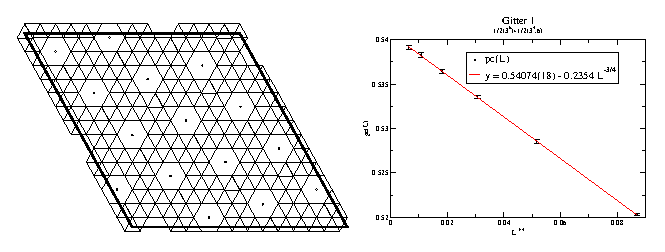
\includegraphics{./Numerik-figs/2-uni-1_fig}
  \caption{Gitter 1: $\frac{1}{2}(3^6)+\frac{1}{2}(3^4,6)$. Das Gitter wiederholt sich erst nach zw\"olf Spalten und Zeilen. In die ``L\"ocher'' wurden zus\"atzliche isolierte Vertices gesetzt.}
\end{figure*}
\begin{figure*}[bp]
  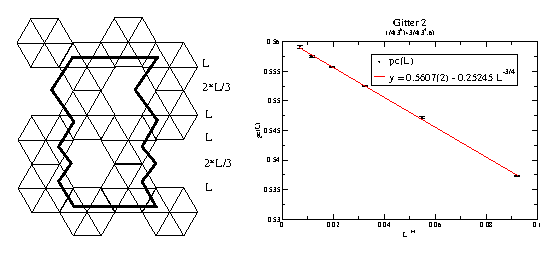
\includegraphics{./Numerik-figs/2-uni-2_fig}
  \caption{Gitter 2: $\frac{1}{4}(3^6)+\frac{3}{2}(3^4,6)$. Die Einheitszelle hat sechs Zeilen und vier Spalten. }
\end{figure*}
\begin{figure*}[p]
  \includegraphics{./Numerik-figs/2-uni-3_fig}
  \caption{Gitter 3:  $\frac{1}{2}(3^6)+\frac{1}{2}(3^3,4^2)$}
\end{figure*}
\begin{figure*}[p]
  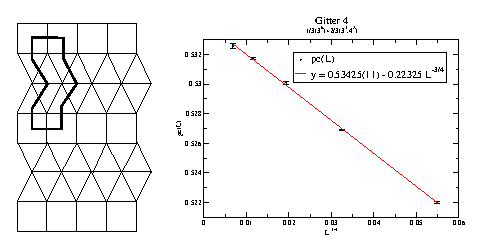
\includegraphics{./Numerik-figs/2-uni-4_fig}
  \caption{Gitter 4: $\frac{1}{3}(3^6)+\frac{2}{3}(3^3,4^2)$}
\end{figure*}
\clearpage
\begin{figure*}[p]
  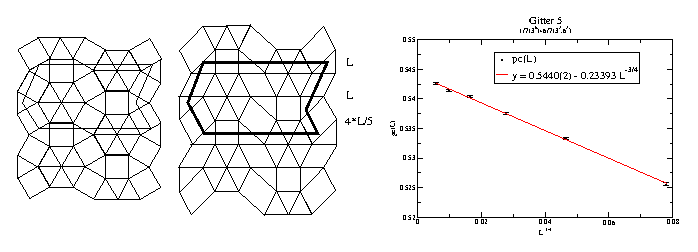
\includegraphics{./Numerik-figs/2-uni-5_fig}
  \caption{Gitter 5: $\frac{1}{7}(3^6)+\frac{6}{7}(3^2,4,3,4)$. Damit eine Zeilenstruktur sichtbar wird, ist es sinnvoll die senkrechten Streifen des Gitter gegeneinander zu verschieben. Die Zeilenl\"angen der Eineheitszelle sind unterschiedlich.}
  \label{fig:appgitter5}
\end{figure*}
\begin{figure*}[p]
  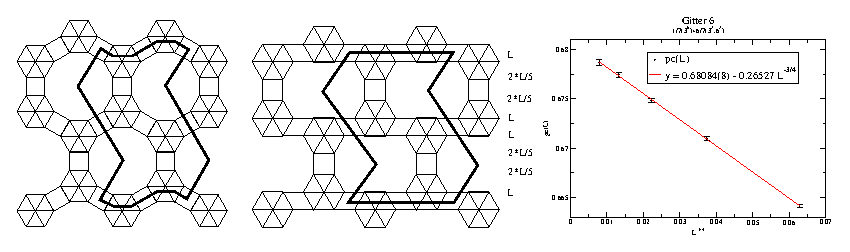
\includegraphics{./Numerik-figs/2-uni-6_fig}
  \caption{Gitter 6:  $\frac{1}{7}(3^6)+\frac{6}{7}(3^2,4,12)$. Die sechseckigen Untereinheiten, bestehend aus sechs Dreiecken, sind auf einem Sechseckgitter angeordnet. Die Untereinheiten sind durch je zwei Kanten verbunden. Leichte Deformation des Gitters erm\"oglicht eine Einteilung in Zeilen. Die L\"angen der Zeilen sind unterscheiden sich. }
\label{fig:appgitter6}
\end{figure*}
\begin{figure*}[p]
  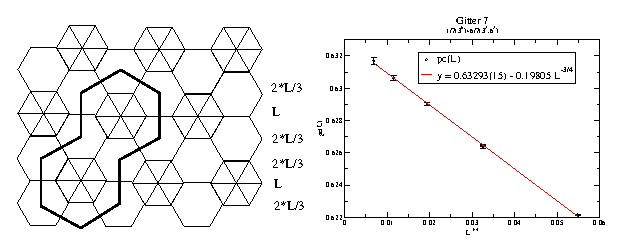
\includegraphics{./Numerik-figs/2-uni-7_fig}
  \caption{Gitter 7: $\frac{1}{7}(3^6)+\frac{6}{7}(3^2,6)$. Der gew\"ahlte Ausschnitt ist nicht der kleinstm\"ogliche. Eine einziges Sechseck, bestehend aus sechs Dreiecken h\"atte ausgereicht.}
\end{figure*}
\clearpage
\begin{figure*}[p]
  \includegraphics{./Numerik-figs/2-uni-8_fig}
  \caption{Gitter 8:  $\frac{1}{2}(3^4,6)+\frac{1}{2}(3^2,6^2)$}
\end{figure*}
\begin{figure*}[p]
  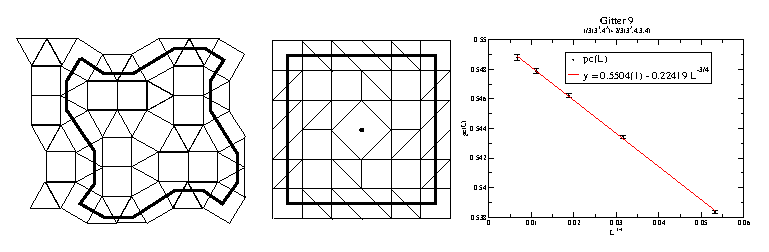
\includegraphics{./Numerik-figs/2-uni-9_fig}
  \caption{Gitter 9: $\frac{1}{3}(3^3,4^2)+\frac{2}{3}(3^2,4,3,4)$. Die Implementierung des Gitters wird erheblich einfacher, wenn es auf ein Quadratgitter transformiert wird, und das zentrale Loch durch einen Geistervertex gef\"ullt ist. Der gew\"ahlte Gitterausschnitt ist f\"unf Spalten breit und f\"unf Zeilen hoch. }
\label{fig:appgitter9}
\end{figure*}
\begin{figure*}[p]
  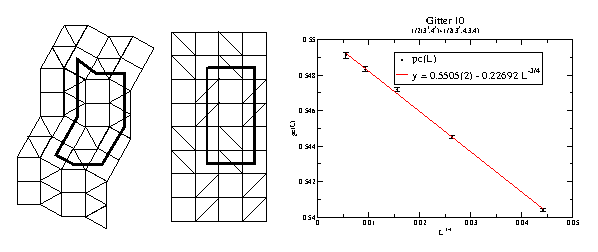
\includegraphics{./Numerik-figs/2-uni-10_fig}
  \caption{Gitter 10:$\frac{1}{2}(3^3,4^2)+\frac{1}{2}(3^2,4,3,4)$. Eine Scherung des Gitters erlaubt die Transformation auf ein Quadratgitter. Die gew\"ahlte Zelle erzeugt bei periodischer Forsetzung aber keinen rechteckigen Gitterausschnitt.}
\label{fig:appgitter10}
\end{figure*}
\clearpage
\begin{figure*}[p]
  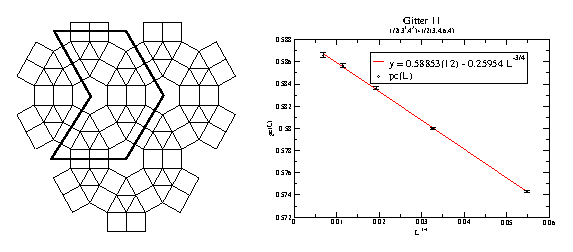
\includegraphics{./Numerik-figs/2-uni-11_fig}
  \caption{Gitter 11:  $\frac{1}{2}(3^3,4^2)+\frac{1}{2}(3,4,6,4)$. Auch bei diesem Gitter l\"asst sich eine Substruktur identifizieren. Je vier Dreiecke bilden ein gro"ses Dreieck, und diese Dreiecke sind auf einem Sechseckgitter angeordnet. Die Einheitszelle besteht aus vier ``Supersechseck-Vertices''.}
\end{figure*}
\begin{figure*}[p]
  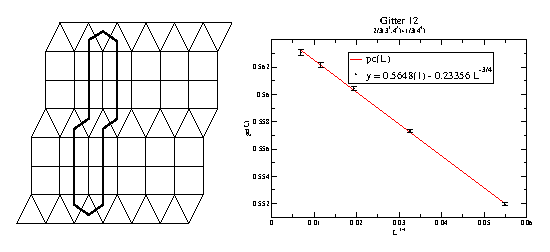
\includegraphics{./Numerik-figs/2-uni-12_fig}
  \caption{Gitter 12:$\frac{2}{3}(3^3,4^2)+\frac{1}{3}(4^4)$. }
\end{figure*}
\begin{figure*}[p]
  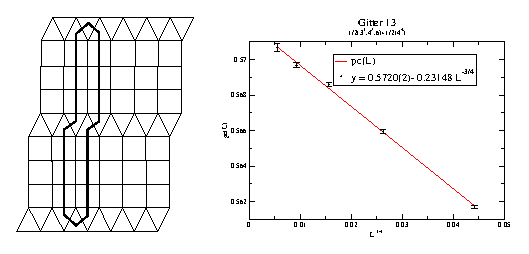
\includegraphics{./Numerik-figs/2-uni-13_fig}
  \caption{Gitter 13: $\frac{1}{2}(3^3,4^2)+\frac{1}{2}(4^4)$. }
\end{figure*}
\clearpage
\begin{figure*}[p]
  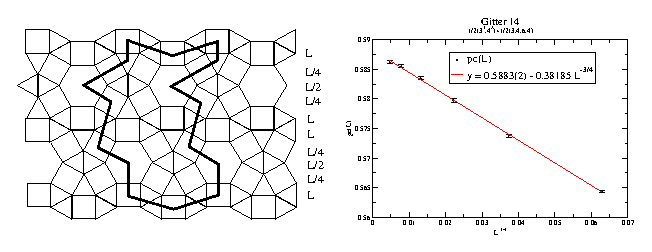
\includegraphics{./Numerik-figs/2-uni-14_fig}
  \caption{Gitter 14: $\frac{1}{2}(3^2,4,3,4)+\frac{1}{2}(3,4,6,4)$. Die Einheitszelle dieses Gitters ist mit vier Spalten und zehn Zeilen sehr gro"s.  }
\end{figure*}
\begin{figure*}[p]
  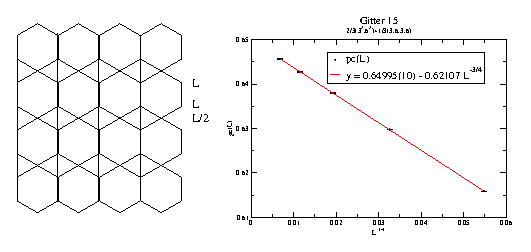
\includegraphics{./Numerik-figs/2-uni-15_fig}
  \caption{Gitter 15: $\frac{2}{3}(3^2,6^2)+\frac{1}{3}(3,6,3,6)$.}
\end{figure*}
\begin{figure*}[p]
  \includegraphics{./Numerik-figs/2-uni-16_fig}
  \caption{Gitter 16: $\frac{1}{2}(3,4,3,12)+\frac{1}{2}(3,12^2)$. Dieses Gitter ist eine Variation des Quadratgitters. Jeder Vertex des Quadratgitters wird durch ein Quadrat und vier Dreiecke ersetzt. Die Struktur, die den Vertex ersetzt, eignet sich als Einheitszelle.}
\end{figure*}
\clearpage
\begin{figure*}[p]
  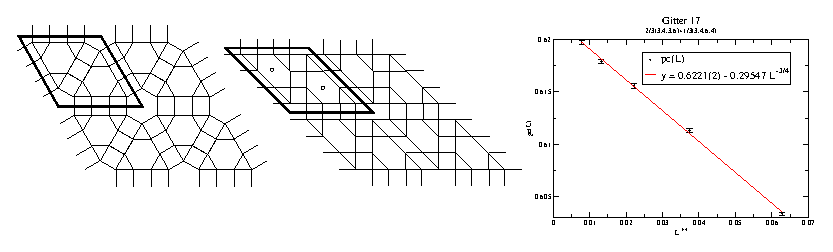
\includegraphics{./Numerik-figs/2-uni-17_fig}
  \caption{Gitter 17: $\frac{2}{3}(3,4^2,6)+\frac{1}{3}(3,4,6,4)$. Das Gitter ist mit dem Sechsecksgitter verwandt. Die Strukturen, bestehend aus einem Sechseck und drei Dreiecken, entsprechen den Sechseckvertices. Zur Implementierung ist es sinnvoll, zwei solche Einheiten zusammenzufassen und zwei Geistervertices in den Sechsecken einzuf\"uhren. Der Ausschnitt ist ein Parallelogramm, und seine Fortsetzung erzeugt ein Parallelogramm und kein Rechteck.}
\end{figure*}
\begin{figure*}[p]
  \includegraphics{./Numerik-figs/2-uni-18_fig}
  \caption{Gitter 18: $\frac{4}{5}(3,4^2,6)+\frac{1}{5}(3,6,3,6)$}
\end{figure*}
\begin{figure*}[tbp]
  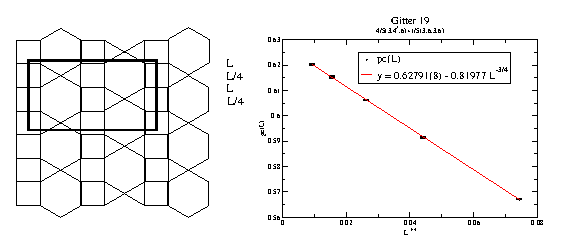
\includegraphics{./Numerik-figs/2-uni-19_fig}
  \caption{Gitter 19:  $\frac{4}{5}(3,4^2,6)+\frac{1}{5}(3,6,3,6)$}
\end{figure*}
\clearpage
\begin{figure*}[tbp]
  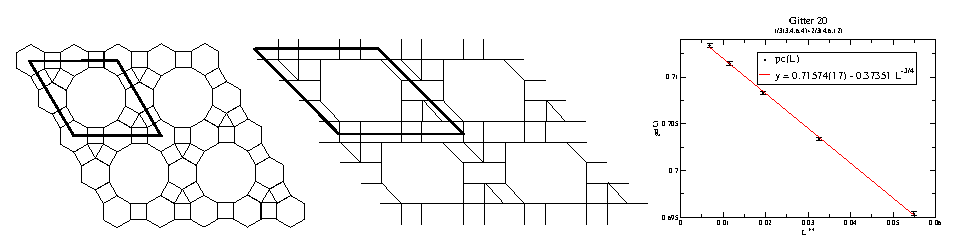
\includegraphics{./Numerik-figs/2-uni-20_fig}
  \caption{Gitter 20: $\frac{1}{3}(3,4,6,4)+\frac{2}{3}(4,6,12)$. Auch dieses Gitter l\"asst sich in Untereinheiten zerlegen, die auf einem Sechseckgitter angeordnet sind. Die Untereinheiten bestehen aus einem Dreieck und drei Quadraten und sind durch Sechsecke miteinander verbunden. Die gew\"ahlte Zelle ist ein Parallelogramm.}
\end{figure*}



\subsubsection{Diskussion}
Unter den 20 2-uniformen Gittern gibt es drei Paare mit identischen Euler-Charakteristiken. Gitter 18 und 19 haben identische Euler-Charakteristiken und sogar identische Vertexkonfigurationen. Trotzdem unterscheiden sich die numerischen Werte f\"ur die Perkolationsschwellen um ca. $7*10^{-4}$, also um mehr als 4 Standardabweichungen. Auch die Gitter 11 und 14, sowie 9 und 10, haben identische Euler-Charakteristik, unterscheiden sich aber in der Anordnung der Polygone um die Vertices und daher in der Vertexkonfiguration. Die ermittelten Perkolationsschwellen der Gitter 11 und 14 bzw. 9 und 10 stimmen innerhalb der Fehlergrenzen \"uberein.




\subsection{Perkolation zuf\"allig dekorierter Gitter}
In Abschnitt \ref{sec:decorated} wurde die Abh\"angigkeit der Perkolationsschwelle eines Gitters vom Bruchteil der dekorierten Gitterplaketten diskutiert. Auch diese Perkolationsschwellen wurden mit dem Algorithmus von Suding und Ziff bestimmt. Das Programm musste dazu entsprechend modifiziert werden. Die L\"ange der Nachbarschaftsvektoren \texttt{nn[i]} muss gleich der Zahl der Nachbarn eines Vertex des vollst\"andig dekorierten Gitters sein. Diese betr\"agt beim Quadratgitter $z=8$, beim Sechseck-Gitter $z=12$, beim Kagom\'e-Gitter $z=10$, beim $3^3,4^2$-Gitter $z=7$ und beim $3,12^2$-Gitter $z=21$. Zu Beginn des Programms wird das undekorierte Gitter erzeugt. Die Eintr\"age der \texttt{nn[i]}, die Verbindungen in einer dekorierten Plakette entsprechen, werden auf \texttt{i} gesetzt und verbinden daher keine Vertices.  Die spanning probability $\bar{p}_{sp}$ wird f\"ur das Gitter der Kantenl\"ange $L$ bestimmt und anschlie"send ein Prozent der Plaketten dekoriert, indem die Eintr\"age \texttt{nn[i]} aller Vertices \texttt{i} auf dem Rand jeder dekorierten Plakette erg\"anzt werden. Dies wird solange wiederholt, bis alle Plaketten dekoriert sind. Die Plaketten werden dabei unabh\"angig und zuf\"allig ausgew\"ahlt. Bei Gittern mit gro"sen Plaketten ist die Dekoration sehr aufwendig. Zur Dekoration eines Zw\"olfecks im $(3,12^2)$-Gitter m\"ussen zum Beispiel $12*9=108$ Eintr\"age der \texttt{nn[i]} erg\"anzt werden.\\
Um die finite-size-scaling Extrapolation zu unendlich gro"sen Gitter durchzuf\"uhren, muss die Simulation auf Gittern verschiedener Gr\"o"se wiederholt werden.

\section{Bestimmung des Erwartungswertes von $\lambda(c_k)$}
\label{sec:noofcomp}
Um die mittleren Euler-Charakteristiken von Gittern mit der Methode aus Kapitel \ref{sec:mixed} zu berechnen, m\"ussen die Erwartungswerte der Gr\"o"sen $\lambda(c_k)$ bestimmt werden. Hier wird das Programm beschrieben, das $\left<\lambda(c_0)\right>$ einer Ecke einer dreidimensionalen Zelle ausrechnet, wenn $3$-Zellen und Fl\"achen mit den Wahrscheinlichkeiten $p_s$ bzw. $p_b$ besetzt werden. Alle anderen Anwendungen sind sehr \"ahnlich. Wenn alle $3$-Zellen und Fl\"achen, die $c_0$ umgeben, besetzt sind, ist $\sigma(c_0)=1$, andernfalls $0$. Wegen dieser Bedingung sind die Beitr\"age der einzelnen Zellen nicht mehr unabh\"angig und jede Konfiguration muss einzeln abgez\"ahlt werden. Das Programm besteht aus einer Schleife \"uber alle m\"oglichen Konfigurationen der Zellen und Fl\"achen, die die Ecke umgeben. Zu jeder Konfiguration wird $\lambda(c_0)$ ausgerechnet und die Wahrscheinlichkeit der Konfiguration bestimmt. 
\\Um aus einer gegebenen Konfiguration aus besetzten $3$-Zellen und Fl\"achen, $\lambda_0$ zu bestimmten, muss die Anordnung der $3$-Zellen und Fl\"achen um $c_0$ bekannt sein. Dazu werden die $3$-Zellen, die $c_0$ umgeben, durchnumeriert und jeder Fl\"ache $c_2$ das Paar von $3$-Zellen, zwischen denen $c_2$ liegt, zugeordnet. Entsprechend werden zu jeder Kante $c_1$ die $3$-Zellen und Fl\"achen gespeichert, die $c_1$ umgeben. Diese Definition der Fl\"achen und Kanten muss per Hand im Quelltext des Programms durchgef\"uhrt werden. 
\\Aus einer vorgegebenen Konfiguration aus besetzten $3$-Zellen und Fl\"achen lassen sich die $\lambda$'s aller $3$-Zellen, Fl\"achen, Kanten nach dem Gleichungen aus Kapitel \ref{sec:mixed} bestimmen. Daraus wird $\lambda_0$ ausgerechnet. Die Wahrscheinlichkeit einer Konfiguration aus $n$ besetzten Zellen und $m$ besetzten Fl\"achen ist $p_s^{n}p_b^{m}(1-p_s)^{N-n}(1-p_b)^{M-m}$, wobei $M$ und $N$ die Gesamtzahl der Fl\"achen bzw. $3$-Zellen ist.  
\\$\lambda(c_0)$ ist eine ganze Zahl zwischen $-M$ und $N$. Um den Erwartungswert von $\lambda(c_0)$ zu bestimmen, muss die Anzahl der Konfigurationen mit $n$ besetzten Vertices, $m$ besetzten Fl\"achen und $\lambda(c_0)=c$ f\"ur alle $0<n\leq N$ und $0<m\leq M$ bekannt sein. Dazu wird ein Feld \texttt{K[N+M+1][N][M]} angelegt und der Eintrag \texttt{K[c+M+1][n][m]} um eins erh\"oht, wenn eine Konfiguration mit $\lambda(c_0)=c$ aus $n$ besetzten $3$-Zellen und $m$ besetzten Fl\"achen gefunden wird. Nachdem alle Konfigurationen abgez\"ahlt sind, erh\"alt man den Erwartungswert $\left<\lambda(c_0)\right>$ durch
\begin{equation}
  \left<\lambda(c_0)\right>_{p_s,p_b}=\sum_{c=-M}^{c=N}\sum_{n=0}^{n=N}\sum_{m=0}^{m=M}c\mathtt{K[c+M+1][n][m]}p_s^np_b^m(1-p_s)^{N-n}(1-p_b)^{M-m}.
\end{equation}